% first draft began 16 September 1999 while in the process of
%     preparing probe for cool down
%
% modifications added 2 May 2000 while in the process of 
%     running the microscope. 
%
% 26 July 2000 - File modified for inclusion into thesis as either
% appendix or chapter.
% to generate this as a simple report, run latex on the file
% expproc.rpt.tex 

% 30 May 2001 with comments from Fred

%\section{Introduction}

\section{Preparing probe for measurements}

Before anything else we make sure that the electrical contacts within 
the probe are good from the room temperature connectors down to the 
connectors inside the vacuum can. After this is done we mount the
sample on the sample holder and align the SQUID and sample. Finally, 
we cool the probe to $4.2\,\kelvin$ and begin measurements.

\subsection{Sample mounting}
\index{sample mounting}

\subsubsection{Preparing to make sample contacts}

The sample must present a flat surface to the SQUID tip. 
There may be no wires or contacts sticking up above the surface of the sample. 
This insures that the SQUID cannot crash into anything during
normal operation. The SQUID (as well as the sample) 
may be destroyed if it crashes. 

Making contacts to a sample this way is non-trivial. One example of how this
has been done is shown in Fig.~\ref{samplecontacts:fig}. The sample chip
is mounted to a silicon or sapphire wafer using stycast epoxy.
For the stycast, we use Black 2850FT with catalyst 24LV\cite{stycast_epoxy}. 
Gold leads are
evaporated such that they overlap the contact pads on the sample chip
surface and make contact to the bottom silicon wafer. Gold or copper
wires can then be attached to using silver paste or indium solder
such that they remain below the surface of the sample chip.

\begin{figure}[p]
\includegraphics{figs/appendixC/fig1.eps}
\caption[Detail of sample contacts]
{Making contacts to the sample such that nothing protrudes 
above the plane of the sample chip}
\label{samplecontacts:fig}
\end{figure}

\subsubsection{Evaporation of contact details}

This applies equally to the contacts made to the sample as well
as to the contacts made to the sample. 
Successful evaporation of gold leads is a straightforward, though
perhaps tedious process. First, we paint photoresist with a small wire
to mask off regions for the evaporated gold. We bake the photoresist
for thirty minutes at eighty degrees centigrade to harden it. After
baking, we double
check under the microscope that photoresist coverage is good and then
mount the sample into the evaporator. We use the ion mill head with the
rotating sample stage, and verify that the sample may rotate freely 
over the evaporator boats. 
The evaporation proceeds according to the following:

\begin{itemize}

\item Ion mill the sample for 30 seconds to clean the surface. 

\item Evaporate $20$ to $50\,\angstrom$ chrome, followed by about 
$2000\,\angstrom$ gold. During the evaporation we 
rotate the sample through the
evaporating material to cover all of the surfaces. 

\item Remove the sample tip from the evaporator and lift off the photoresist. 

\item Evaporated gold does not typically stick to the stycast epoxy so we
use silver paint to connect over the stycast.

\item Attach wires to these leads using silver paste or indium 
solder. 

\end{itemize}

\subsubsection{Mounting sample into probe}

The entire assembly mounts with Apeizon N vacuum grease\cite{apiezon}
to the sapphire cylinder of the
sample holder in the probe. 
The sapphire cylinder is clamped into a gold coated 
copper cold finger. This cold finger is thermally sunk to the helium bath
through 
copper heat sinking. Around the sapphire cylinder a solenoid is wound
which applies magnetic field to the sample. 

\subsection{SQUID mounting}
\index{SQUID!mounting}
\label{app:squid_mounting}

We prepare the SQUID tip in a similar fashion to that of the
sample. 
This is done by taking a
\squid\ chip (as cut from the Hypres delivered wafer) 
and mounting it to a sapphire cone with stycast epoxy. 
At this point the SQUID chip is square and we grind it down
until it is circular and the same size as the tip of the
sapphire cone (about $1\,\mm$). 

Grinding is started using a Dremel
tool with an emery wheel. Grind the SQUID under a microscope to observe
the grinding process. The emery wheel removes fairly large 
chunks from the SQUID, so at some point is unsatisfactory to 
grind the SQUID further. The grinding is completed using a
polishing wheel. 

Contacts are made to the \squid\ chip by
evaporating gold onto the contact pads and over and down the sides. 
This gold should cover the stycast epoxy and go down to the sapphire cone. 
Indium wets to sapphire at about $300^{\circ}\,\mathrm{C}$ and can be used to 
contact the evaporated gold. We have also had good luck
using a combination of silver paste and silver paint.
Small copper or gold wires are then
used to contact the indium and connect to the rest of the probe wiring.
This layout is sketched in Fig.~\ref{samplecontacts:fig}. 
We have tried many different ways to make these contacts: silver paint and
paste and various solders. In all of the cases, the big problem is 
thermal cycling. The SQUID must be thermal cycled in vacuum, otherwise
ice crystals form that eventually break the contacts free. 
This makes testing in a dip probe problematic because the SQUID is not
put in vacuum, nor is the Bellcore Dewar neck large enough to make
a vacuum can that could contain the SQUID holder. 
A good solution would be to make a special probe to insert
into a standard experimental Dewar. We have not done this. 
We dip test the SQUID a couple of times and verify that it
works with the electronics anyway.

The longest
lasting SQUID survived for approximately eighteen months, and had indium
contacts, it crashed into a sample which destroyed it. 
We gingerly test the SQUID in the dip probe and
make sure that it thermal cycles slowly. We only thermal cycle it 
one or two times this way. 
Once it works, we mount the SQUID in the probe and only thermal cycle
it in vacuum.
The contacts should work okay with this procedure.
With this method we are careful of the wires themselves and
examine them for  kinks that may break
upon subsequent thermal cycling. 
\index{SQUID!mounting!thermal cycling}
The \squid\ will likely
be thermal cycled many times before any useful data is taken so its 
important to get this to work properly. 

\begin{figure}[p]
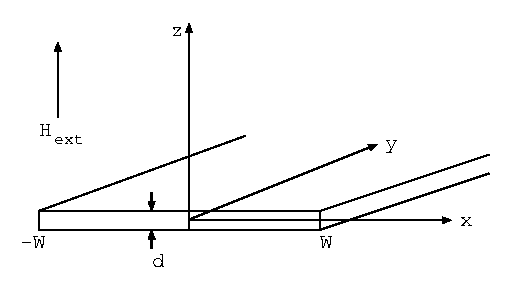
\includegraphics{figs/appendixC/fig2.eps}
\caption[Detail of SQUID contacts]
{Contacts made to the SQUID such that nothing protrudes
above the \squid\ tip.}
\label{fig:squidtipcontacts}
\end{figure}

The SQUID mounts into the probe similarly to the sample. The \squid\  
sits on the end of a sapphire cone which is clamped into a gold coated
copper cold finger. This copper cold finger is thermally sunk to the helium
bath by means of a copper heat sinking, separate from the sample.
Provided that the
vacuum in the probe is good  the sample and the \squid\
should both be thermally isolated from each other. In practice the \squid\
needs considerable heat sinking to maintain a constant temperature.

\index{alignment!SQUID-sample!z-control}
\index{SQUID-sample alignment!z-control}
The \squid\ cold finger is mounted in a Delrin plate which holds the \squid\ 
above the sample. The \squid\ height above the sample can be controlled
with a $z$-wedge. Moving this wedge in and out raises and lowers
the SQUID above the sample. 
There is considerable backlash in this mechanism and
it cannot be relied upon for measurements nor can it be calibrated. 


\subsection{\squid\ and sample contacts}
\index{SQUID!mounting!contacts to probe}
\index{sample mounting!contacts to probe}
\index{pinouts!room temperature}

After mounting, we check the all of the contacts from the vacuum can up to the
room-temperature flange. Typical pinouts are listed in 
Table~\ref{rtcontacts:table} along with typical 
resistances at room temperature.

%% pinouts.tex
%  pinouts of ssm probe in long table format 

\begin{longtable}{c||lr|r|r|r}
\caption[Microscope room temperature flange pinouts]
{Microscope room temperature flange pinouts with typical resistance
values for the vacuum can at $4.2\,\kelvin$, $77\,\kelvin$ and room
temperature.}\\
\label{rtcontacts:tablej}
& & & & &\\
\endfirsthead
\caption[]{\emph{Room temperature flange pinouts continued}}
\\ \hline
\endhead
\\ \hline
\multicolumn{6}{r}{\emph{continued on next page}}
\endfoot
\\ \hline
\endlastfoot
& \multicolumn{2}{c|}{SQUID} & $4.2\,\kelvin$ & $77\,\kelvin$ & $300\,\kelvin$ \\
\hline
A & transformer & & & & \\
B & transformer & & & & \\
\end{longtable}


\begin{table}
\begin{tabular}{c||lr|lr|lr}
\multicolumn{7}{c}{\textbf{Probe pinouts at room temperature}}\\
\hline \hline
& \multicolumn{2}{c|}{\squid} & \multicolumn{2}{c|}{Temp} & \multicolumn{2}{c}{He Level} \\ 
\hline\hline
A &                 &    &               & $V+$     &                & $V+$\\
B & \raisebox{.2in}[.2in]{transformer}     &    &               & $V-$     &                & $V-$\\ \cline{2-3}
C &                 &    &  \raisebox{.2in}[.2in]{sample thermo} & $I+$    & \raisebox{.2in}[.2in]{He level meter} & $I+$\\
D &  \raisebox{.2in}[.2in]{feedback coil}   &    &               & $I-$     &                & $I-$\\ \cline{2-7}
E &                 &                    &          &                & NC & \\
F &  \raisebox{.2in}[.2in]{$I_{\mathrm{bias}}$}     &               &  \raisebox{.2in}[.2in]{sample heater} &  \raisebox{.2in}[.2in]{$33.5\,\Omega$} & NC & \\ \cline{2-5}
G &  & & & $V+$            & NC & \\
H &  \raisebox{.2in}[.2in]{coil} &  \raisebox{.2in}[.2in]{$11.4\,\Omega$}          & &  $V-$             & NC & \\\cline{2-3}
J & &  &  \raisebox{.2in}[.2in]{\squid\ thermo}& $I+$    & NC & \\
K &  \raisebox{.2in}[.2in]{\squid\ heater} &  \raisebox{.2in}[.2in]{$40.8\,\Omega$}    & & $I-$      & NC & \\
\hline \hline
  & \multicolumn{2}{c|}{Sample 1} & \multicolumn{2}{c|}{Sample 2} & & \\ 
\hline\hline
A & & $V+$    & NC & & & \\
B & & $V-$    & NC & & & \\
C & \raisebox{.2in}[.2in]{plastic thermo} & $I+$    & NC & & & \\
D &  & $I-$    & NC & & & \\ \cline{2-5}
E & NC             &     & &  & & \\
F & NC             &     & \raisebox{.2in}[.2in]{solenoid} & \raisebox{.2in}[.2in]{$15\,\Omega$}          & & \\ \cline{4-5}
G & NC             &     & NC & & & \\ 
H & NC             &     & NC & & & \\
J & NC             &     & NC & & & \\
K & NC             &     & NC & & & 


\end{tabular}

\caption[Room temperature flange pinouts at room temperature]
{Room temperature flange pinouts at room temperature. All resistances listed are those
measured at room temperature}
\label{rtcontacts:table}
\end{table} 

\begin{table}
\begin{tabular}{c||lr|lr|lr}

\multicolumn{7}{c}{\textbf{Probe pinouts in liquid nitrogen}}\\
\hline \hline
& \multicolumn{2}{c|}{\squid} & \multicolumn{2}{c|}{Temp} & \multicolumn{2}{c}{He Level} \\ 
\hline\hline
A &                 &    &               & $V+$     &                & $V+$\\
B & \raisebox{.2in}[.2in]{transformer}     &    &               & $V-$     &                & $V-$\\ \cline{2-3}
C &                 &    &  \raisebox{.2in}[.2in]{sample thermo} & $I+$    & \raisebox{.2in}[.2in]{He level meter} & $I+$\\
D &  \raisebox{.2in}[.2in]{feedback coil}   &    &               & $I-$     &                & $I-$\\ \cline{2-7}
E &                 &                    &          &                & NC & \\
F &  \raisebox{.2in}[.2in]{$I_{\mathrm{bias}}$}     &               &  \raisebox{.2in}[.2in]{sample heater} &  \raisebox{.2in}[.2in]{$30.0\,\Omega$} & NC & \\ \cline{2-5}
G &  & & & $V+$            & NC & \\
H &  \raisebox{.2in}[.2in]{coil} &  \raisebox{.2in}[.2in]{$8.0\,\Omega$}          & &  $V-$             & NC & \\\cline{2-3}
J & &  &  \raisebox{.2in}[.2in]{\squid\ thermo}& $I+$    & NC & \\
K &  \raisebox{.2in}[.2in]{\squid\ heater} &  \raisebox{.2in}[.2in]{$30.0\,\Omega$}    & & $I-$      & NC & \\
\hline \hline
  & \multicolumn{2}{c|}{Sample 1} & \multicolumn{2}{c|}{Sample 2} & & \\ 
\hline\hline
A & & $V+$    & NC & & & \\
B & & $V-$    & NC & & & \\
C & \raisebox{.2in}[.2in]{plastic thermo} & $I+$    & NC & & & \\
D &  & $I-$    & NC & & & \\ \cline{2-5}
E & NC             &     & &  & & \\
F & NC             &     & \raisebox{.2in}[.2in]{solenoid} & \raisebox{.2in}[.2in]{$15\,\Omega$}          & & \\ \cline{4-5}
G & NC             &     & NC & & & \\ 
H & NC             &     & NC & & & \\
J & NC             &     & NC & & & \\
K & NC             &     & NC & & & 

\end{tabular}

\caption[Room temperature flange pinouts at $77\,\kelvin$]
{Room temperature flange pinouts at $77\,\kelvin$. 
All resistances are measured at $77\,\kelvin$}
\label{table:nitrogen_pinouts}
\end{table} 


\begin{table}

\begin{tabular}{c||lr|lr|lr}

\multicolumn{7}{c}{\textbf{Probe pinouts in liquid helium}}\\
\hline \hline
& \multicolumn{2}{c|}{\squid} & \multicolumn{2}{c|}{Temp} & \multicolumn{2}{c}{He Level} \\ 
\hline\hline
A &                 &    &               & $V+$     &                & $V+$\\
B & \raisebox{.2in}[.2in]{transformer}     &    &               & $V-$     &                & $V-$\\ \cline{2-3}
C &                 &    &  \raisebox{.2in}[.2in]{sample thermo} & $I+$    & \raisebox{.2in}[.2in]{He level meter} & $I+$\\
D &  \raisebox{.2in}[.2in]{feedback coil}   &    &               & $I-$     &                & $I-$\\ \cline{2-7}
E &                 &                    &          &                & NC & \\
F &  \raisebox{.2in}[.2in]{$I_{\mathrm{bias}}$}     &               &  \raisebox{.2in}[.2in]{sample heater} &  \raisebox{.2in}[.2in]{$28.0\,\Omega$} & NC & \\ \cline{2-5}
G &  & & & $V+$            & NC & \\
H &  \raisebox{.2in}[.2in]{coil} &  \raisebox{.2in}[.2in]{$2.2\,\Omega$}          & &  $V-$             & NC & \\\cline{2-3}
J & &  &  \raisebox{.2in}[.2in]{\squid\ thermo}& $I+$    & NC & \\
K &  \raisebox{.2in}[.2in]{\squid\ heater} &  \raisebox{.2in}[.2in]{$27.8\,\Omega$}    & & $I-$      & NC & \\
\hline \hline
  & \multicolumn{2}{c|}{Sample 1} & \multicolumn{2}{c|}{Sample 2} & & \\ 
\hline\hline
A & & $V+$    & NC & & & \\
B & & $V-$    & NC & & & \\
C & \raisebox{.2in}[.2in]{plastic thermo} & $I+$    & NC & & & \\
D &  & $I-$    & NC & & & \\ \cline{2-5}
E & NC             &     & &  & & \\
F & NC             &     & \raisebox{.2in}[.2in]{solenoid} & \raisebox{.2in}[.2in]{$1.7\,\Omega$}          & & \\ \cline{4-5}
G & NC             &     & NC & & & \\ 
H & NC             &     & NC & & & \\
J & NC             &     & NC & & & \\
K & NC             &     & NC & & & 

\end{tabular}

\caption[Room temperature flange pinouts at $4.2\,\kelvin$]
{Room temperature flange pinouts at $4.2\,\kelvin$. 
All resistances are measured at $4.2\,\kelvin$}
\label{table:helium_pinouts}
\end{table}

 

\subsection{Sample and \squid\ alignment}
\index{SQUID-sample alignment!horizontal}
\index{alignment!SQUID-sample!horizontal}

Once both the sample and \squid\ are mounted in the probe and their contacts
are okay, we
align them with respect to each other. We bring the two close to each other
using the $z$-wedge and by adjusting the \squid\ mounting screws so that 
the SQUID is 
level with respect to the plane in which the sample moves. We do this using 
a stereo microscope. We then
repeat the process with the sample. 

Next we attach the stepper motor drive to the probe and use the joystick 
control to move the sample around while watching with the microscope. 
we adjust the \squid\ and sample until they are aligned such that the
\squid -sample separation does not change over the entire range of the 
sample's motion. 

\index{SQUID-sample alignment!coordinates}
\index{alignment!SQUID-sample!coordinates}
Once the alignment is complete we record the coordinates. Generally the center
of the sample is taken as $(0,0)$ in the coordinate system of the 
\squidbox. Relative to this location record the
upper-left and lower-right coordinates of the scan and save these
values in the computer. Note the physical relationship
with respect to the stepper motor coordinate system (used in the 
SQUIDBox) and the tick marks on the $x,y,z$ pushrods. 

\subsubsection{Maximum scanning range}

\index{alignment!sample slider!travel range}
The $x,y$ stage has a maximum travel range. 
The tall push rod should not be raised to less than $40\,\mm$,
on its millimeter scale because
parts of the sliding mechanism can 
run into stationary parts of the probe and wreck the scanning
mechanism. 
Always check for
obstructions to the scanning mechanism before scanning, and note of any
features that might interfere with the scanning. 

\index{alignment!sample slider!grabbing}
\index{sample slider!mechanical grabbing}
After many thermal cycles, the Delrin housing for the positioning mechanism
may begin to catch the sample holder because it shifts out of 
alignment. If this occurs, the housing should be
fully disassembled, and then reassembled paying strict attention to tolerances
on each side, to ensure that the sample holder may slide freely. Problems with
sliding may not manifest at room temperature, and may require dipping the 
scanning mechanism 
and housing into liquid nitrogen in order to test properly. 

After recording 
these numbers the \squid\ can be moved to a safe position for the
rest of the procedure. Back the \squid\ far away from the sample and 
move the sample so that the \squid\ is not positioned over anything important.
Generally we move the \squid\ over a gold pad and position it there. 
Typical values for all of these alignment parameters are shown in 
Table~\ref{alignprms:table}. 

\begin{table}
\begin{tabular}{l|rrr|rr}  
                &  \multicolumn{3}{c|}{pushrods} & \multicolumn{2}{c}{steppers} \\
                &     tall (mm) & short (mm) & $z$-wedge (mm) &  $x$ & $y$  \\ \hline    
 Centered       &   72          &   37       &  5           &  0 & 0 \\
 Upper Left     &   68          &   30       &  5           & 154490 & 41650 \\
 Lower Right    &   106         &   45       &  5           & -207133 & -40587 \\
 Safety         &   89          &   42       &  20          & -44000  & -44000 
 
\end{tabular}
\caption{Typical values for the alignment parameters of the \squid\
and the sample.}
\label{alignprms:table}
\end{table}

\index{vacuum can}
After verifying that the contacts are good and aligning the \squid\ and sample
we move
the probe into the screened room. Be extremely careful
of the wires when doing this as they are prone to catch on things and break.
Generally we recheck all the contacts before tightening the screws for the
vacuum can. 
\index{lead can}
There is a lead liner for the vacuum can which is supposed to help act as a
magnetic shield. This lead liner has never been used primarily 
for two reasons. First
fitting everything into the vacuum can is a 
difficult proposition and requires some contortion to make it work;
there is simply no room for the lead can. Second
the lead can may trap flux and frustrate, rather than help, our
attempt to reduce the ambient flux.

\section{Pumping down and leak checking}

\index{diffusion pump}
\index{leak checking}
Evacuate the probe using the diffusion pump station. 
The diffusion pump has a base pressure of about 
$2 \times 10^{-6}\,\mathrm{torr}$. 
We have achieved this pressure using the diffusion pump alone, but only
once. It took about two days to reach this pressure so just be patient. There
are so many crevices that virtual leaks are a big problem, so its hard
to tell if there is a real leak or not. Generally we pump for 24 hours until 
the
probe pressure reaches about $10^{-5}\,\mathrm{torr}$.

At this point it is a 
good time to leak check the probe. There are so many things which can go
wrong and the entire procedure takes so much time that we have found it
beneficial to leak check the probe every time it is used. However, at room
temperature the probe generally proves to be leak tight. Important things to
check at this point are the large indium O-ring sealing the vacuum can
as well as the fittings at the top. The connectors on the cold flange are known
to leak, but generally only leak when in liquid nitrogen or helium. 
Check them to be safe. In order to finish leak checking it is necessary to 
cool the probe in liquid nitrogen. 

\section{Pre-cooling in liquid nitrogen}

\index{pre-cooling}
\index{cooling!nitrogen}
The leak checking procedure can be finished by putting the probe into the 
experiment Dewar and cooling with \lnit. 
The most important thing is to cool the probe slowly. We have 
found that cooling the probe quickly results in 
vacuum leaks opening up on the cold flange. Begin with an empty Dewar.
Make sure the Dewar contains no nitrogen nor debris 
at the 
bottom. Any debris in the bottom may block the transfer lines when you
later
try to blow the nitrogen out of the Dewar. 

Clamp the small fill line to the side of the vacuum can before continuing.

If the Dewar is warm simply lower the probe into the Dewar, and bolt the 
flange to the top of the Dewar. Reattach the diffusion pump the probe and 
continue to pump on the probe and monitor the pressure. We now start
to cool the probe by trickling liquid nitrogen into the Dewar. Do this slowly.
we prefer to use the small storage Dewar, pressurized to  $5\,\mathrm{psi}$. 
At this pressure
the nitrogen transfers slow enough rate is slow enough that the 
probe is not stressed. If you use a large 
storage Dewar the pressure is $22\,\mathrm{psi}$ 
and it is easy to transfer nitrogen too quickly. 
\index{cooling!nitrogen!transfer time}%
The nitrogen transfer should take from fifteen minutes to a half hour. 

We never lower the probe into the Dewar if there is already liquid nitrogen
in the Dewar. This puts a lot of thermal stress on the vacuum
joints and causes leaks. We have tried lowering the probe slowly into a
nitrogen bath and it does not work. 

Watch the pressure in the probe as you transfer the nitrogen. 
It should drop continuously.
Sometimes the pressure may jump up and then drop back down. This is okay and
just means that a virtual leak opened up. If the pressure shoots up and 
cannot be pumped down this means that a leak has opened up on the cold end
of the probe. 

\index{leaks!cold!nitrogen}
Its necessary to try and find the leak. Let the probe fully cool in nitrogen. 
The thermometers work at nitrogen temperature
so you can tell that the probe is fully cooled. Once the probe is fully cooled,
pull it out of the Dewar and leak check it immediately before it has time to 
warm up.
The leak can often be found this way.
Leaks are often found in the solder joints for the electrical 
feed throughs on the cold flange.

\index{leaks!cold!reproducibility}
Before trying to repair the leak, let the probe warm fully to room temperature
and repeat the leak checking procedure. Liquid nitrogen leaks frequently
go away at room temperature. Additionally the leaks 
do not often repeat, so try
again.  Cool very slowly into nitrogen, slower than before, 
and see what happens.

If no leaks develop you can proceed to cool with liquid helium. If the leaks
do not go away they must be assessed. Any loss of vacuum in the probe means
that the thermal isolation between the \squid\ and the sample will be 
degraded.
If the leak is small enough that we can pump on it continuously and keep 
a 
vacuum around $10^{-5}\,\mathrm{torr}$ or smaller
then we do so. If the leak is too large then it will
have to be repaired. 

\section{Cooling with liquid helium}

\index{pinouts!$77\,\kelvin$}
Before moving on, we check the 
electrical contacts in the probe again.
See table~\ref{table:nitrogen_pinouts} for typical resistances at
$77\,\kelvin$.
 This is important
because we can save a lot of time if we find a bad contact here. 
If there is a bad contact we pull the probe out to make
a repair and are careful to blow the liquid nitrogen out of the Dewar before
we pull the probe out. If we do not do this, the nitrogen will stay
in the Dewar for a long time, and we do not want to lower the probe into
nitrogen bath. Instead, we
only want to trickle nitrogen slowly around the probe.

\index{sample slider!$77\,\kelvin$}
In addition to checking the electrical contacts at $77\,\kelvin$, 
we also check the
scanning mechanism and verify that it can move smoothly over
the full range of required travel. If the mechanism binds up, it will
be necessary to open the probe and figure what is wrong. It may be
necessary to disassemble the entire Delrin housing and reassemble to
make sure that the mechanism operates smoothly. 

\index{cooling!helium}
The trick to cooling with liquid helium 
is to cool as slowly as possible. Since the plastic has
very low thermal conductivity, a long wait is required to draw all of the
heat out of the plastic. From $77\,\kelvin$ to $4.2\,\kelvin$, 
cooling takes between
two and three hours. 

\index{cooling!exchange gas}
It is also necessary to put helium into the vacuum can as exchange gas, 
otherwise the plastic will never cool. At $77\,\kelvin$, we put about 
$50\,\mathrm{mTorr}$ 
of helium gas. We have also used hydrogen as exchange gas, but it freezes
out at about $11\,\kelvin$ and then it is impossible to cool the probe below
$11\,\kelvin$. 

Blow the liquid nitrogen out of the Dewar.

Begin the liquid helium transfer, while monitoring the temperature.
The \squid\ will cool the fastest because it is the best heat sunk. 
We monitor closely the plastic temperature and use that as a guide. 
As long as the plastic continues to cool, everything is fine. In
general we do not want to condense helium into the Dewar until
the plastic has cooled to $4.2\,\kelvin$. This process does not require much
effort, but must be monitored to insure that the transfer continues
slowly. 

It is essential that we cool the probe cool uniformly and slow enough so
that the plastic temperature remains the same as the vacuum can 
temperature. It is easy to cool the vacuum can to $4.2\,\kelvin$ while the 
plastic temperatures remains quite high ($30-40\,\kelvin$). In this case, 
the helium exchange gas condenses on the inside surface of the can
and the plastic cease to cool at any reasonable rate. If this happens, we
allow
any liquid helium to boil off, and the vacuum can is allowed to
warm above $4.2\,\kelvin$, before attempting to re-cool the probe. LakeShore 
germanium thermometers are mounted on the sample, SQUID, cold flange and 
plastic to monitor the temperature during cooling. 

\section{Finding the sample}

Once the probe is at $4.2\,\kelvin$, 
verify that the \squid\ is working properly and check the electrical
contacts. Typical resistances at $4.2\,\kelvin$ are shown in 
table~\ref{table:helium_pinouts}.

\index{alignment!finding sample at $4.2\,\kelvin$}
Because of thermal contraction, the sample shifts inside the can
when it is cooled to $4.2\,\kelvin$. This makes it somewhat challenging to find
the sample once everything else is set to go. We have
found that it's easiest
to put an AC field into the sample solenoid, use a lock-in amplifier
to look at the same frequency in the SQUID electronics output
and scan around. There are always gradients in the 
DC remnant field which sometimes make it difficult to search for the sample by
using a DC field into the sample solenoid. 

\index{alignment!SQUID-sample!z-control!$4.2\,\kelvin$}
\label{app:squid_sample_alignment}
We do not move too close to the sample initially. It is possible to knock
the sample off the sample mount if the SQUID tip catches 
an edge of the sample. 
However, it is often difficult to find the sample location with out 
moving somewhat closer. We always move closer to the
sample while watching the \squid\ output. If the \squid\ touches the 
sample, it will unlock, and if we are gentle, we can back away
and there should be no problems.

It is generally easy to find the sample using this method and then
we recheck the coordinates.

Once the sample is located, we bring the SQUID 
closer to it and try to get as close
as possible. This is tricky because the sample may not be level any 
longer. We start in the middle of the sample, and move in until I just
touch. Then we back the SQUID 
away and attempt to move around using the joystick
control. We move over the entire scan range and 
make sure that the \squid\ and sample do not touch. If all is well, 
we try a scan and it should appear as we expect. It is 
difficult to know
how close the SQUID is to the sample or if the sample is
even level with respect to the plane of the SQUID. The best way
to figure the SQUID height above the sample is to scan an image which
has features of known size. Unfortunately, not all samples have
such features.

\section{Day to day operation}

The Dewar hold time is about twelve hours. So, we transfer helium every
twelve hours. We fill the 
liquid nitrogen jacket every 
24 hours. At this point, 
aside from making sure the cryogens are full, there is not
too much to worry about. 

If the vacuum is poor, we may need to pump on the probe 
continuously. 

\subsection{Holding}

If no data is to be taken, the probe can safely be left for 24 hours
between helium transfers. In this time, the probe will warm to 
about $20\,\kelvin$ to $30\,\kelvin$. 
This amount of heating is not a problem, and the 
probe can safely be re-cooled to $4.2\,\kelvin$ for the resumption of data
collection.

It takes approximately 48 hours for the probe to warm to $100\,\kelvin$. 
At this
temperature, the probe should be held in liquid nitrogen to 
insure that it does
not warm any further. It will also be necessary to cool in nitrogen to 
$77\,\kelvin$ before re-cooling to $4.2\,\kelvin$. 
Warming above $77\,\kelvin$ has proven to cause faults
arising from 
thermal stresses to the electrical contacts and the 
vacuum seals. 

\subsection{Scanning}

\index{sample slider!scanning friction}
During scanning, it is essential to mitigate the effects of heating
due to friction in the slider mechanism. This heating causes not only
the sample to warm slightly, but also the SQUID. 
We wish to hold the SQUID to 
as constant a temperature as possible, otherwise the 
critical current will drift, which in turn causes the SQUID voltage
to drift, shifting the measured output from the SQUID electronics.

%The effects of the heating can clearly be seen in data taken without
%any temperature control, as shown in Fig.~\ref{fig:heatingimage}. 

%
% cut this for lack of a good figure. 
%
%\begin{figure}
%\caption[Images of SQUID data affected by friction]
%{(a) A zero background magnetic image taken with the SSM. 
%The gradient in the image is due to the drift in the SQUID temperature. 
%(b) A vertical line cut through the image showing the drift with temperature. }
%\label{fig:heatingimage}
%\end{figure}

This effect has been measured more carefully by warming the SQUID and noting
the change in output, as discussed in section~\ref{sec:squid_vs_temperature},
p.~\pageref{sec:squid_vs_temperature} and shown in 
\FigRef{fig:squid_vs_temperature}.

\index{temperature control!SQUID}
\index{temperature control!sample}
Neocera LTC-21 Cryogenic Temperature controllers are used to control 
both the SQUID and sample temperatures during scanning. The control 
parameters
for the temperature controllers must be set each time and are usually 
quite different between data runs. This is because we often change 
the heat sinking
or the quality of the vacuum is different between
data runs. Once stabilized the temperature controllers do an effective
job of maintaining both the SQUID and sample temperatures to 
within $0.01\,\kelvin$. Typically the SQUID is operated at a temperature of 
$4.8\,\kelvin$. 

\section{Warming up}

\index{warming probe}
We allow the probe to warm to at least $77\,\kelvin$ before pulling
it out of the Dewar.
 Otherwise thermal stress can cause vacuum 
leaks. Typically we let the probe sit in the Dewar and warm up 
as slowly as possible. 

When the probe is at $77\,\kelvin$ or greater, we pull it out of the
Dewar and let it warm to room temperature. we do not break the vacuum
until it has fully warmed to room temperature (even deep inside the
can). Otherwise, ice will form inside the can. The ice crystals 
seem to degrade the contacts; especially the SQUID contacts. 
Typically, wait twenty-four hours for the probe to warm to room 
temperature from $77\,\kelvin$.
 

\section{Vacuum leak information}
\index{leak checking!cold}

This appendix contains information about finding and repairing the
vacuum leaks. This is information that was sent to me from John Markus
of Rick
Newrock's group at the University of Cincinnati. 

\begin{quotation}

%From johnm@physics.uc.edu Fri Sep 17 12:05:36 1999
%Date: Tue, 19 Jan 1999 10:45:39 -0500 (EST)
%From: John Markus <johnm@physics.uc.edu>
%To: anielsen@squid.umd.edu
%Cc: John Markus <johnm@physunc.phy.uc.edu>
%Subject: vacuum leaks

Hi Aaron,

Sorry to hear that you still have some leaks, but relieved that it seem to
be the feed throughs rather than a weld. (by the way, we've recently opened
our probe and the cold flange patch weld is on the inside of the vacuum
can in case you haven't noticed it yet).  The following may or may not
help but here is an outline of the technique I've used to get successful
joints when reusing those low temp. feed throughs and brass flanges.  I prefer
to use a hot plate rather than a heat gun because the temp is easier to
control and it's easier to inspect and work on the part without heating up
my hands and face.

\begin{enumerate}
\item support the brass flange with feed through connector side up on a 
$\frac{7}{8}\,\inch$ OD.
by $\frac{1}{2}\,\inch$ long copper pipe on a hot plate.

\item increase the hot plate temp slowly until the old solder melts

\item by grabbing a few pins with needle nose pliers, remove the feed through
from the flange and quickly wipe away any extra solder from the feed through. 
I find a cloth rag works well or you can clean up the surface with a
soldering iron.  Just try to have the sides and step tinned without any
lumps so it will fit back into the flange

\item clean up the brass flange while it is still hot, I use Stay-Clean
liquid flux on a cotton swab to remove extra solder

\item  re-tin the side surfaces of the flange if necessary

\item melt new solder in the step of the flange so there is a nice continuous
bead of molten solder all the way around the ring.  Our solder%
\footnote{This low temperature solder is Cerrolow 117 or 137. The number
refers to the melting point in Centigrade.} is in
awkward squares so we melt is on a soldering iron and let drops fall on a
glass plate to get usable flat drips that can be cut with a razor blade
and applied to the part using tweezers

\item apply Stay-Clean liquid flux around the feed through with a cotton swab

\item  with needle nose pliers set the feed through into position on the flange. 
If it doesn't really fit do to some extra solder blobs that were difficult
to clean, preheat the feed through with a heat gun until the solder flows and
then install the feed through

\item  set a small mass on the pins of the feed through to keep it from ``floating''
up on the solder. I use a $\frac{3}{4}\,\inch$ long piece of 
$\frac{1}{2}\,\inch$ OD solid copper rod.

\item  add solder to any gaps around the perimeter of the feed through

\item  turn off the hot plate and don't move the assembly until it is cool
enough to touch and hold in your hand

\item  wash the assembled parts (maybe in baking soda solution) to neutralize
and remove the nasty acid flux. then dry completely with compressed air.

\end{enumerate}

I don't recall the melting temp of the solder we used and I don't have any
info on those feed throughs but I would guess they can handle a temp higher
than $117\,\mathrm{F}$ 
so you may want to try another solder.  The black filler on
those is probably some glass-filled epoxy and since it is a solder type
connector, should be able to handle rather high temperatures.  If you have
a spec. sheet on them it may recommend a solder to use or at least a maximum
temp. (If you find out anything I'd appreciate a note about it)  Maybe you
shouldn't try a higher temp unless you've got some spares sitting around,
I guess their pretty expensive--like \$100 for one tested to 
$4\,\kelvin$ by the company.

Leak checking is always annoying and cold leak checking is even worse.  I
assume you've got some mass spectrometer vacuum leak detector tuned to
$^4\mathrm{He}$.  
My number one rule and advice to students is Do Not use too much test
gas.  If you know you have a leak then careful, minimum He application is
key.  He atoms are very fast and with large amounts flying around its very
hard to pin-point a leak.  As a test gas applicator, I've taken a damaged
needle valve from the gas handling system of a deposition chamber and
attached to it a thin piece of $\frac{1}{16}\,\inch$ 
OD flexible copper tubing about $6\,\inch$ long.
I set the He flow rate with the needle valve by watching the bubbles in a
beaker of water when the tip of the wand is submerged (for fine leaks
maybe 1-2 bubbles per second).  Then move the wand around one suspect
joint or part of joint at a time waiting a short time before moving to the
next joint.  Since He rises in air and I assume the probe is hanging
vertically, start at the top and work your way down.  For leak checking
while at $\ell \mathrm{N}_2$ temps, try incrementally 
lowering a small Dewar of $\ell \mathrm{N}_2$ off the
probe and testing those joints just above the liquid level.  This does two
things for you, 1. it helps keep the joints cold and 2. it block random He
from possible leaks below the liquid level.  You may need to use a higher
He flow rate to overcome the boiling $\ell \mathrm{N}_2$ gas flow around 
the test area.  I
have a 10 liter Nalgene Dewar (Fisher Scientific cat no. 10-194-100d \$225)
that I raise and lower on the stationary hanging probe with a lab jack. 
This Dewar is small enough to be manageable yet deep enough to submerge the
cold flange, except for the double feed through.  (if your lab doesn't have
something similar, check in the physics departments lecture demonstration
equipment for one you could borrow.)

Good luck and keep me posted on your progress.  If any of the above is
unclear or you have other questions just send me a note. - John

\end{quotation}

\pagebreak



